% Created 2025-09-06 Sat 20:03
% Intended LaTeX compiler: pdflatex
\documentclass[presentation]{beamer}
\usepackage[utf8]{inputenc}
\usepackage[T1]{fontenc}
\usepackage{graphicx}
\usepackage{longtable}
\usepackage{wrapfig}
\usepackage{rotating}
\usepackage[normalem]{ulem}
\usepackage{amsmath}
\usepackage{amssymb}
\usepackage{capt-of}
\usepackage{hyperref}
\usetheme{default}
\author{Mr. Maxwell}
\date{\today}
\title{unit 1: atoms, isotopes, and ions}
\hypersetup{
 pdfauthor={Mr. Maxwell},
 pdftitle={unit 1: atoms, isotopes, and ions},
 pdfkeywords={},
 pdfsubject={},
 pdfcreator={Emacs 29.3 (Org mode 9.6.15)}, 
 pdflang={English}}
\begin{document}

\maketitle
\begin{frame}{Outline}
\tableofcontents
\end{frame}



\begin{frame}[label={sec:org3d84294}]{Unit: atoms, isotopes, and ions}
\begin{block}{Lesson: atomic structure}
\begin{itemize}
\item \alert{objective:} label an electron cloud diagram of the atom showing the locations of electrons, protons, and neutrons
\end{itemize}
\begin{block}{diagram:}
\begin{center}
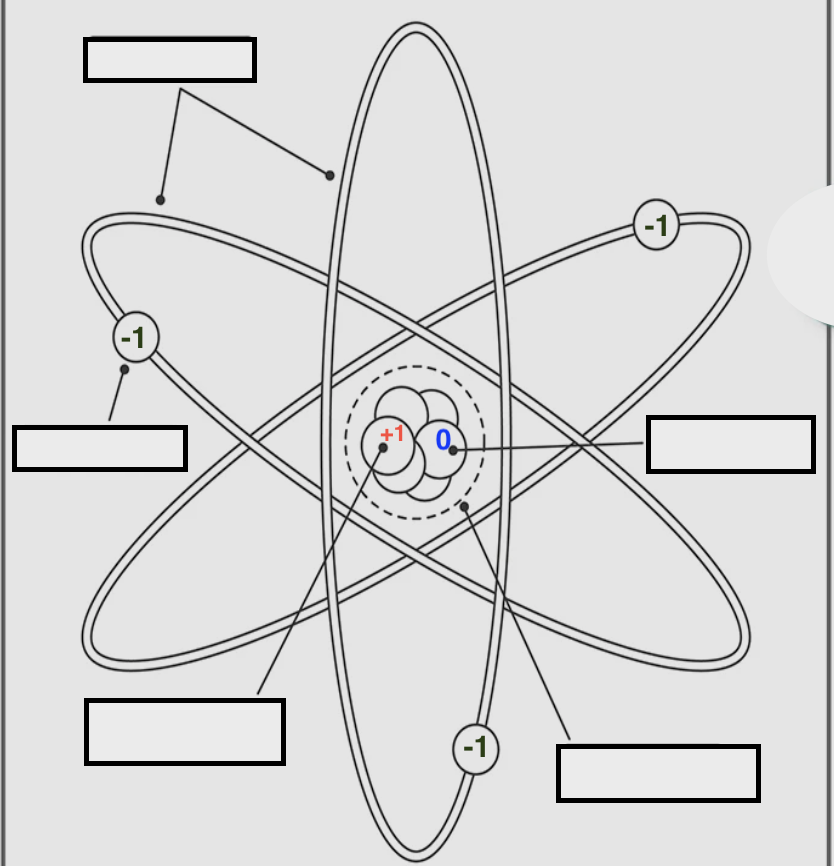
\includegraphics[width=0.7\textwidth]{./atomNotes.png}
\end{center}
\end{block}

\begin{block}{charges of particles}
\begin{center}
\begin{tabular}{ll}
subatomic particle & charge\\[0pt]
\hline
proton & positive(+)\\[0pt]
neutron & neutral(0)\\[0pt]
electron & negative(-)\\[0pt]
\end{tabular}
\end{center}
\end{block}
\end{block}
\end{frame}
\end{document}
